%%%%%%%%%%%%%%%%%%%%%%%%%%%%%%%%%%%%%%%%%%%%%%%%%%%%%%%%%%%%%%%%%%%%%%
\documentclass[12pt]{article}
\usepackage{setspace}
\usepackage[numbers,round]{natbib}
\bibliographystyle{apalike}
\usepackage{changebar}
\usepackage{tabularx}
\usepackage{graphicx}
\usepackage[margin=1in]{geometry}
\usepackage{comment}
\usepackage{matlab-prettifier}
%\usepackage{siunitx}
%\usepackage{seqsplit}
\textheight 9in
\textwidth 6.5in
%\topmargin -1in
%\oddsidemargin -.2in


%%%%%%%%%%%%%%%%%%%%%%% New commands

% These are handy commands you can use to create consistent and correct
% special characters, units, and expressions.
\newcommand{\etal}{{\em et al.}}
\newcommand{\etc}{{\em etc.}}
\newcommand{\eg}{{\em e.g.,}}
\newcommand{\ie}{{\em i.e.,}}
\newcommand{\cpp}{C{\raisebox{0.5ex}{\tiny++}}}
\newcommand{\degrees}{{$^{\circ}$}}
\newcommand{\muv}{${\rm \mu V}$}
\newcommand{\ohm}{$\Omega$}
\newcommand{\sft}{${\rm ft^2}$}


\begin{document}
	
	


\title{HW1: Molecular Biophysics}
\author{Jake Bergquist, u6010393 }
\maketitle

\section{Q1}
\subsection{a}
I found the nitric oxide synthase heme domain at 1.65 A resolution in Bos taurus found via X-ray crystallography on rcsb.org. The catelog ID is 1D0C. The amino acid sequence of chain B is as follows:


  SRAPAPATPHAPDHSPAPNSPTLTRPPEGPKFPRVKNWELGSITYDTLC\\
  AQSQQDGPCTPRRCLGSLVLPRKLQTRPSPGPPPAEQLLSQARDFINQY\\
  YSSIKRSGSQAHEERLQEVEAEVASTGTYHLRESELVFGAKQAWRNAPR\\
  CVGRIQWGKLQVFDARDCSSAQEMFTYICNHIKYATNRGNLRSAITVFP\\
  QRAPGRGDFRIWNSQLVRYAGYRQQDGSVRGDPANVEITELCIQHGWTP\\
  GNGRFDVLPLLLQAPDEAPELFVLPPELVLEVPLEHPTLEWFAALGLRW\\
  YALPAVSNMLLEIGGLEFSAAPFSGWYMSTEIGTRNLCDPHRYNILEDV\\
  AVCMDLDTRTTSSLWKDKAAVEINLAVLHSFQLAKVTIVDHHAATVSFM\\
  KHLDNEQKARGGCPADWAWIVPPISGSLTPVFHQEMVNYILSPAFRYQP\\
  DPW\\

\subsection{b}
With the search criteria Thrombin, and homo sapiens I found that the thee most recent structures available are 6GBW, 6FJT, and 6EVV as of 9/3/19.

\section{Q2}
\subsection{a}
Position g in the structure has the highest proportion of amino acids that are charged at 4/5 residues at this position. The first of those is an arginine. It is at the amino terminal end which implies a pKa near 9.04. Even if this were a non terminal amino acid it would have a pKa of ~ 12.48. Thus this amino acid will be positively charged. The two are lysines which have a side chain pKa of 10.79, resulting in a positive charge. The next is a glutamic acid which has a side chain pKa of 4.25, resulting in a negative charge at neutral pH. The last amino acid in this position is a leucene which does not ionize as a side chain and thus will have a neutral charge.

\subsection{b}
For the next part I used the Table 1.1 from lecture notes 1.b. I added the Hydrophobicity of the side chain measurements to find the total energy for the transfer from water to an non-polar solvent.\\
i) Ala-Thr-Ser: -3.65 + 14.74 + 18.23 = 29.32 kJ/mol\\
ii) Phe-Ile-Trp: -8.57 + -16.71 + -5.84 = -31.12 kJ/mol\\


\section{Q3}
There appears to be a fairly linear relationship between volume and hydrophobicity scale number for the amino acids with a hydrophobic side chain (A V I L M F Y W) with tyrosine sitting as a bit of an outlier. Additionally if C R and K are excluded then the remaining amino acids (some charged, some polar) (D N E Q H) also show a fairly linear relationship. The fitline shown in Figure~\ref{fig:trend} is approximated for the entire dataset. The slope is roughly 80 units volume per hydrophobicity scale number. When compared to the surface area vs free energy of transfer graph from the lecture notes it appears that both graphs depict a similar motif, with two groups having distinct linear trends, one group with most of the non-polar side chains and one trend with most of the polar side chains. The trend in the lecture notes graph has a strikingly similar slope by eye (the relevant axes are flipped) however the data seems to be  better fit to a linear relationship in the lecture notes graph than in Figure~\ref{fig:trend}
\begin{figure}[H]
	
	\centering
	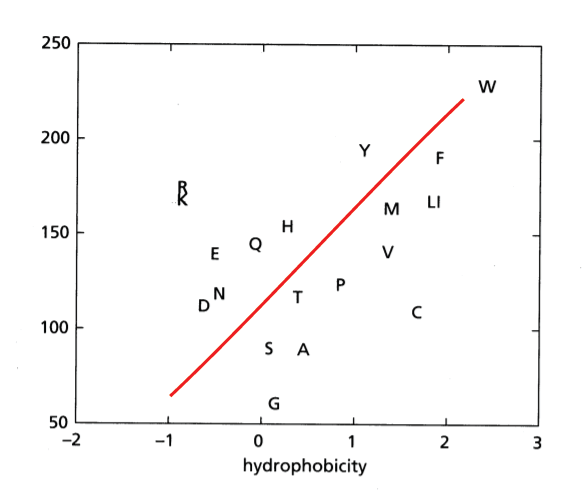
\includegraphics[width=.95\textwidth]{Trend.png}
	
	\caption{Approximate trendline fit to the presented data.}
	\label{fig:trend}
\end{figure}

\section{Q4}
\subsection{a}
The following matlab code was used to calculate the stoke's radius using the given parameters. The results are shown in Table~\ref{tab1}.
\begin{lstlisting}[style=Matlab-editor]
D = [21,10,7,1,0.8,0.7,0.07].*1e-6;%cm^2/s 
M = [18,32,180,13680,3500,6800,345000];

%y = 6pinr

%D = kT/y

%solve for r
%D = kT/6pinr
%r = kT/(6*pi*D*n)

%body temperature is ~37 celsius = ~310 Kelvin
T = 310;%K
%Boltzman's constant
k = 1.38e-23;%J/K
%Convert k to be in units of cm
%k = 1.38e-23 kg m^2/s^2 K * 100cm/m * 100 cm/m
k = k * 100 * 100;%kg cm^2 / s^2 K
%Viscocity of water at 310 K
n = 0.6913;%mPa/s
%convert to proper units
%n = 0.6931 mPa/s = 0.0006931 Pa/s = 0.0006931 kg/m s^3
% * 100cm/c = 0.06931 kg/cm s^3
n = n/1000 * 100;%kg/cm s^3

for ind = 1:length(D)
r(ind) = (k*T)/(6*pi*n*D(ind));
end

alpha = 0.462;
offset = 2e12;
testR = M.^(alpha);

figure(1);clf();hold on; 
scatter(M,testR/offset,'r');
scatter(M,r,'b');
set(gca,'yscale','log')
set(gca,'xscale','log')
legend({'fit data','measured data'});
xlabel('Molecular Weight (log)');
ylabel('Stokes Radius (log)');
\end{lstlisting}

\begin{table}[h]
	\caption{Calculated Stoke's Radius}
	\centering
	\begin{tabular}{|r|r|r|r|} \hline
		
		Material&D (cm2/s) 10-6& M (g/mole)& r (cm)\\
		\hline
		water& 21& 18& 1.56e-12\\
		oxygen& 10& 32& 3.28e-12\\
		glucose& 7& 180&4.69e-12 \\
		ribonuclease& 1 13& 680&3.28e-11 \\
		lactoglobulin& 0.8& 35,000& 4.10e-11\\
		hemoglobin& 0.7& 68,000& 4.69e-11\\
		collagen& 0.07& 345,000& 4.69e-10\\
		\hline
	\end{tabular}
	\label{tab1}
\end{table}

subsection{b}
Figure~\ref{fig:fit} shows the measured and fit data. An exponential term of 4.62 was used to acchieve this fit. I could not get the fit data to match the measured data without a scaling factor of $2*10^{12}$ that I divided the fit data by to bring it into the same range as the measured data. I am not sure of the spurce of this scale missmatch, perhaps an error in my calculations, but after re formulating the calculations several times I cannot seem to  find the error.

\begin{figure}[h]
	
	\centering
		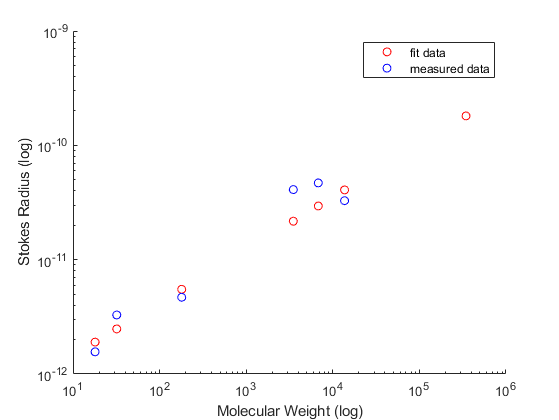
\includegraphics[width=.95\textwidth]{fitData.png}
	
	\caption{Calculated Stoke's radius vs molecular weight (blue) and fit data (red).}
	\label{fig:fit}
\end{figure}

\section{Q5}
\subsection{a}
We know that $k = {EA}/L$ for the lognitudional spring constant of a rod or rod like object where k is the spring constant/stiffness, E is the young's modulus, A is the cross sectional area, and L is the length. Thus for this muscle the spring constant is k = 40 * 1000 / 100 = 400 MPa*mm. Doing some unit conversion/homogenation to clear things up 1 Pa = 1 $\frac{kg}{m*s^2}$. $1 MPa = 1*10^6 Pa$. Thus $400 MPa*mm = 4*10^8Pa*mm = 4*10^5 Pa*m = 4*10^5 kg/s^2$.

\subsection{b}
Assuming that the weight is pulling directly down on the face of the muscle towards earth (the vector of the force is in line with gravity) then the Force exerted by this weight would be $F = m*a = 10 kg * 9.8 m/s^2 = 98 N$. We can calculate the change in length ($\delta L$) according to : $\frac{F}{A} = E\frac{\delta L}{L}$ by solving for $\delta L$. We know all of the other terms. This rearranges to $\delta L = \frac{FL}{AE} = \frac{98 N*0.1 m}{0.001 m^2 * 4*10^7 Pa} =   \frac{9.8 kg*m^2 / s^2}{ 4*10^4 m*kg/s^2} = 2.45*10^{-4}m = 0.245 mm$. The fractional extension is $\delta L/L$ which is 0.00245.

\subsection{c}
Like in A, the stiffness is calculated as $k = {EA}/L$ . In this case this comes out to $k = 2.3GPa*20 nm^2 / 1 \mu m = 46 GPa*nm^2/\mu  m = 4.6*10^7 Pa*nm^2/\mu  m = 4.6*10^{-11}Pa*m^2/\mu  m = 4.6*10^{-5}Pa*m = 4.6*10^{-5} kg/s^2$

\subsection{d}
Given the cross sectional area of $20 nm^2 = 2*10^{-17}m^2$ per filament, and a length of 100 mm (0.1 m) and young's modulus of 2.3 GPa for actin, we can calculate a stiffness for this actin filament. This would be $k = E * A/L = 2.3 GPa * \frac{2*10^{-17}m^2}{0.1m} = 2.3 GPa * 2*10^{-18}m = 4.6*10^{-18} GPa m = 4.6*10^{-9} kg/s^2 $. Because these are parallel springs we can add their stiffness to get the total stiffness of the muscle and use that to calculate the total young's modulus of the muscle. At $10^{15}$ filaments per square meter there are $10^{15} filaments/m^2 * 1000 mm^2 = 10^{15} f/m^2 * 0.001 m^2 = 10^{12} filaments$ in this muscle. Thus the stiffness is $10^{12} * 4.6*10^{-9}kg/s^2 = 4.6*10^3kg/s^2$. If we plug this into our stiffness calculation and solve for the youngs modulus we get $E = k*(L/A) = 4.6*10^3 kg/s^2 *(0.1 m/ 0.001 m^2) = 4.6*10^5 Pa = 0.46 MPa$. This value is one order of magnitude less than the decribed Young's modulus for muscle, implying that there are stiffer elements to a muscle than if it were to be made solely of actin. However within one order of magnitude is fairly close, implying that actin does contribute to a major portion of a muscle's young's modulus.
%%%%%%%%%%%%%%%%%% Correct Bibliography Style

\section{Q6}
There are three potential methods to calculate the overlap concentration, either using the end-to-end distance, radius of gyration, or both. By first computing the size of the polymer then dividing the mass by the size we can achieve the concentration, assuming ideal conditions. Finally the intrinsic viscosity is related to the overlap concentration according to $c^* = 1/[n]$ where $c^*$ is the concentration, and $[n]$ is the intrinsic viscosity.

If we assume that there are no effects on size other than the nearest neighbor relationships for this polymer then the mean squared end to end length is $<r> = Nb^2$ where N is the number of units and b is the bond length. Thus the end to end length (the RMS end to end length) is $\sqrt{Nb^2} = sqrt{1000 * (.3nm)^2} = sqrt{1000 * (3*10^{-10}m)^2} = 9.49*10^{-9} m$. If we assume a globular protein then we can approximate its volume with $\frac{4}{3}\pi r^3$ where r is half the RMS end to end distance. This gives us a volume of $4.47*10^{-25}m^3$. To calculate the concentration we take the molecular weight divided by the volume, which is $90,000 Da / 4.472*10^{-25}m^3 = 1.50*10^{-19} g / 4.472*10^{-25}m^3 = 3.34*10^{5} g/L$.\\
If instead we use the radius of gyration, which is calculated using the mean squared end to end length according to $R_g = <r>/6 = (1000 * (3*10^{-10}m)^2)/6 = 1.50*10^{-17} m$. Again by using this radius to calculate a volume ($1.41*10^{-50} m^3$) and diving the mass by this volume we get the excluded concentration, this time a value of $1.06*10^31 g/L$. This is a strikingly different number.
Both of these calculations are done assuming an ideal conditions protein in which steric hindrances are ignored and the protein is considered to be in an ideal solution at the theta point. As to which one makes more sense and is realistic I would initially guess the Radius of Gyration, however the resultant value seems much larger than would be expected. A quick check using a generic density of proteins $~1g/cm^3 = 1000 g/L$ (Fischer H, Polikarpov I, Craievich AF. Average protein density is a molecular-weight-dependent function. Protein Sci. 2004;13(10):2825–2828. doi:10.1110/ps.04688204) shows much closer agreement to the method using the RMS end to end distance.

The intrinsic viscocity is the inverse of the excluded volume under theta/ideal conditions. Thus for these calculations that comes out to either $2.99*10^{-6} L/g$ or $9.46*10^-{32}L/g$ for RMS end to end distance or radius of gyration respectively
.


\end{document}








